% \documentclass[modern]{aastex63}
\documentclass[twocolumn]{aastex63}

\shorttitle{RR Lyrae in the Pal 5 stream}
\shortauthors{People et al.}
\newcommand{\sa}[1]{{\color{teal} SP: #1}}

% Load common packages
\usepackage{microtype}  % ALWAYS!
\usepackage{amsmath}
\usepackage{amsfonts}
\usepackage{amssymb}
\usepackage{booktabs}

\usepackage{graphicx}
\usepackage{color}

\newcommand{\documentname}{\textsl{Article}}
\newcommand{\sectionname}{Section}
\renewcommand{\figurename}{Figure}
\newcommand{\equationname}{Equation}
\renewcommand{\tablename}{Table}

% Missions
\newcommand{\project}[1]{\textsl{#1}}

% Packages / projects / programming
\newcommand{\package}[1]{\textsl{#1}}
\newcommand{\acronym}[1]{{\small{#1}}}
\newcommand{\github}{\package{GitHub}}
\newcommand{\python}{\package{Python}}
\newcommand{\emcee}{\project{emcee}}

% For referee
\newcommand{\changes}[1]{{\color{red} #1}}

% Stats / probability
\newcommand{\given}{\,|\,}
\newcommand{\norm}{\mathcal{N}}

% Maths
\newcommand{\dd}{\mathrm{d}}
\newcommand{\transpose}[1]{{#1}^{\mathsf{T}}}
\newcommand{\inverse}[1]{{#1}^{-1}}
\newcommand{\argmin}{\operatornamewithlimits{argmin}}
\newcommand{\mean}[1]{\left< #1 \right>}

% Unit shortcuts
\newcommand{\msun}{\ensuremath{\mathrm{M}_\odot}}
\newcommand{\kms}{\ensuremath{\mathrm{km}~\mathrm{s}^{-1}}}
\newcommand{\mps}{\ensuremath{\mathrm{m}~\mathrm{s}^{-1}}}
\newcommand{\pc}{\ensuremath{\mathrm{pc}}}
\newcommand{\kpc}{\ensuremath{\mathrm{kpc}}}
\newcommand{\kmskpc}{\ensuremath{\mathrm{km}~\mathrm{s}^{-1}~\mathrm{kpc}^{-1}}}

% Misc.
\newcommand{\bs}[1]{\boldsymbol{#1}}

% Astronomy
\newcommand{\DM}{{\rm DM}}
\newcommand{\feh}{\ensuremath{{[{\rm Fe}/{\rm H}]}}}
\newcommand{\df}{\acronym{DF}}
\newcommand{\logg}{\ensuremath{\log g}}
\newcommand{\Teff}{\ensuremath{T_{\textrm{eff}}}}

% TO DO
\newcommand{\todo}[1]{{\color{red} TODO: #1}}


\begin{document}

\title{Kinematics of the Palomar 5 stellar stream from RR Lyrae stars}

\author[0000-0003-0872-7098]{Adrian~M.~Price-Whelan}
\affiliation{Center for Computational Astrophysics, Flatiron Institute,
             Simons Foundation, 162 Fifth Avenue, New York, NY 10010, USA}
\affiliation{Department of Astrophysical Sciences,
             Princeton University, Princeton, NJ 08544, USA}
% \email{aprice-whelan@flatironinstitute.org}
% \correspondingauthor{Adrian M. Price-Whelan}

\author[0000-0002-6330-2394]{Cecilia~Mateu}
\affiliation{Departamento de Astronom\'ia, Facultad de Ciencias, Universidad de la Rep\'ublica, Igu\'a 4225, 14000, Montevideo, Uruguay}
    

\author{Giuliano~Iorio}
\affiliation{Institute of Astronomy, University of Cambridge, Madingley Road, Cambridge CB3 0HA, UK}

\author{Sarah~Pearson}
\affiliation{Center for Computational Astrophysics, Flatiron Institute,
             Simons Foundation, 162 Fifth Avenue, New York, NY 10010, USA}

\author{Vasily~Belokurov}
\affiliation{Institute of Astronomy, University of Cambridge, Madingley Road, Cambridge CB3 0HA, UK}

% \author{more people?}


\begin{abstract}
\todo{This is just placeholder text!}
% Context
Stellar streams are important.
The Palomar 5 stellar stream is a prototypical example: It connects back to the progenitor cluster.
RR Lyrae-type (RRL) stars are useful because they are standard candles and their distances can be inferred with small errors ($\sim7\%$)
% Aims
While the Pal 5 cluster is known to host a small number (5--7) of RRL stars, only two RRL stars have since been found in the long tidal tails that form the Pal 5 stream.
% Methods
Here we use a large catalog of RRL stars released as a part of Gaia DR2 to search for RRL stars in the Pal 5 stream.
By building a probabilistic model of the cluster and stream in proper motion and distance, we find XX RRL consistent with being members of the stream.
% Results
The number of Pal 5 RRL is therefore XX times larger in the tails than in the remnant cluster: This changes our interpretation of ...blah.
% Conclusions
Stuff.
\end{abstract}

\keywords{globular clusters: individual: Palomar 5 -- 
Galaxy: halo --
stars: variables: RR Lyrae --
Galaxy: structure}

\section{Introduction} \label{sec:intro}

Globular clusters are destroyed as they orbit within the Milky Way.
The $\sim$150 bound globular clusters we presently see throughout the Galaxy \citep{Harris2010} are therefore thought to be surviving relics of a much larger initial population, most of which were destroyed (primarily) through a combination of relaxation / evaporation and gravitational shocking from the disk and bulge \citep[e.g.,][]{Gnedin:1997, Gnedin:2014}.
As stellar systems are destroyed---i.e., as stars are tidally stripped from their progenitor---the tidal debris forms tails of matter that both lead and trail the remnant cluster, producing a stellar stream that may persist even after the progenitor is fully destroyed \citep[e.g.,][]{Johnston:1996, Eyre:2011}.

Stellar streams are useful objects because they almost\footnote{More precisely, the phase-space distribution of stars along a stream encodes the orbital history of the progenitor system \citep[e.g.,][]{Sanders:2013}.} delineate the past and future trajectory of their progenitor system, offering information about orbits that can be used to infer the mass distribution from the single kinematic snapshot of the Galaxy that we are afforded \citep[e.g.,][]{Johnston:1999, Binney:2008, Eyre:2009, Sanders:2013, PriceWhelan:2014, Bonaca:2018}.
Many globular cluster stellar streams have been discovered over the last few decades \citep[see, e.g.,][]{Grillmair:2016, Shipp:2018}, in large part because of large-area, deep, multi-band imaging surveys such as the Sloan Digital Sky Survey \citep[SDSS;][]{York:2000}, Pan-STARRS PS1 survey \citep{Chambers:2016}, and Dark Energy Survey \citep{DES:2016}.
A subset of the known streams have been precisely characterized and further studied \citep[e.g.,][]{PriceWhelan:2018, Malhan:2018, Shipp:2019} using kinematic data from the recent data release 2 (\DR{2}) of the \Gaia\ mission \citep{Gaia:2016, Gaia:2018}.
Of the currently known $\sim$60 candidate stellar streams found throughout the Milky Way, few have known progenitor systems.
Conversely, of the $\sim$150 known globular clusters, only $\lesssim 20\%$ have purported tidal tails \citep[e.g.,][]{Leon:2000, Kundu:2019}, but even these are mostly low density and tenuous \citep[as might be expected, e.g.,][]{Balbinot:2018}.
A prominent exception to these statements is the Palomar 5 (Pal 5) globular cluster and stream.

The Pal 5 stream---at a heliocentric distance of $d \sim 20~\kpc$---was discovered using early SDSS imaging, which reached well below the main sequence turnoff of the stream over a large area surrounding the cluster \citep{Odenkirchen:2001, Rockosi:2002}.
Since then, radial velocities have been measured for a handful of giant branch stars in the cluster and along the stream \citep{Odenkirchen:2002, Odenkirchen:2009, Ibata:2017}, and deeper imaging data has been used to map the tails at higher signal-to-noise \citep{Bernard:2016, Ibata:2016, Bonaca:2019}.
The detailed but still limited kinematic data for Pal 5 has made it a canonical example of tidal destruction and a useful tool for constraining Galactic structure.
For example, using the sky track and radial velocity information, the stream has been used to measure the enclosed mass of the Milky Way \citep{Kuepper:2015, Bovy:2016}.
Using deep photometry, the density variations along the stream have been used to place limits on the abundance of massive substructures in the Galactic halo \citep{Erkal:2017}.

However, a number of peculiar aspects of the stream still remain unexplained in detail.
For example, the leading and trailing tails have significantly different total star counts and lengths \citep{Dehnen2004, Bernard:2016}, and the stream track, width, and density vary significantly over the full extent of the stream \citep{Ibata:2016, Bonaca:2019}.
Given that Pal 5's pericenter is well within the Galactic disk ($r_{\textrm{peri}} \sim 7$--$8~\kpc$), these features could be a sign of perturbations from molecular clouds \citep[e.g.,][]{Amorisco:2016}, interaction with the Galactic bar \citep[e.g.,][]{Pearson:2017}, signatures of past dark matter subhalo encounters \citep[e.g.,][]{Erkal:2017}, or some combination of all of these effects.
Mapping the stream in all six phase-space dimensions---i.e., combining deep photometry with radial velocity, distance, and proper motion measurements---will enable and motivate improved dynamical models of the stream and more precise constraints on the Galactic mass distribution \citep[e.g.,][]{PriceWhelan:2013}.
However, at its present distance, main sequence stars are barely detected and have large astrometric uncertainties in \Gaia\ \DR{2}, and other stellar tracers (e.g., giant branch stars) are not numerous enough or precise enough distance indicators to provide useful relative distance information along the stream.
% Enter RR Lyrae-type stars.

\todo{Cecilia: write this paragraph? you probably have some canned text? - (In progress, CM.}
RR Lyrae stars (RRLs) are pulsating horizontal branch giants intrinsically more luminous than main sequence stars, but about $\sim 10,000$ time less numerous. They can be reliably identified based on their photometric variability alone, with little to no contamination from other types of variable stars, and are well known standard candles. Their distances can be estimated based on photometric data alone by means of their period-luminosity relation, with distance errors that go from $\sim8\%$ in the optical to as low as 3\% in the infrared \citep{Neely2017,Sesar2017a}. At its current distance, Pal~5's horizontal branch is bright enough $\G\sim17.3$ to be observed by \Gaia, so it's full extent can be traced and kinematic properties measured with RRLs.
%meaning we can measure kinematic properties of the full stream...
\citep{Ibata:2017} found some RRL in pal 5, but no proper motions.
This is useful for modeling...
Many stream candidates found in RRL alone \citep{Mateu:2018}.

In this Article, we construct a probabilistic model for kinematic properties of RRLs in the vicinity of the Pal 5 stream to determine membership probabilities and thus map the distance and proper motion trends in the stream.
In \sectionname~\ref{sec:data}, we describe the source RR Lyrae catalog we use to search for Pal 5 members.
In \sectionname~\ref{sec:membership}, we implement a probabilistic membership model to identify candidate members of the stream using distance and astrometric information.
In \sectionname~\ref{sec:results}, we ...


\section{Data} \label{sec:data}

% From \Gaia~DR2 we have combined the two available RRL catalogues: the Specific Objects Study \citep[SOS][]{Clementini2018} and vari-classifier \citep[VC][]{Holl2018,Rimoldini2018}. The resulting VC+SOS catalogue contains a total of 228\,904, with all-sky coverage down to the mission's limiting magnitude $G=20.7$. After filtering out stars with contaminated photometry \verb+phot_bp_rp_excess_factor+>2 or null, as recommended in \citep{Rimoldini2018}, the VC+SOS catalogue contains a total of 175\,164 RR Lyrae. For the 122\,747 in SOS, which have undergone extensive light curve fitting, periods, amplitudes and other fitting parameters have been provided by \citet{Clementini2018}. The remaining 52\,417 stars (from the VC catalogue) did not have enough data points in \Gaia~DR2 to go into the SOS pipeline, so periods and other fitting parameters are not yet available for these stars.  

To search for RRLs in the vicinity of Pal 5, we use a catalog of RRL stars from the PS1 survey that spans $\sim$3/4 of the sky (all sky north of declination $\delta > -30\degr$) and contains 61\,795 RRLs identified from their variability \citep{Sesar2017b}.
In detail, the \emph{bona fide} RRLs in the catalog were classified using multi-epoch data in the $grizy$ photometric bands, with a typical number of 12 observations per filter, and has a limiting magnitude $r\sim21$ (corresponding to $G~21$ for the typical colors of RRLs).
Periods and amplitudes in all five bands are available for all stars in this catalog. 
We have chosen to use this catalog instead of the recently released \Gaia~RRL catalogs \citep[VariClassifier and Specific Object Studies][]{Holl2018, Rimoldini2018, Clementini2018} as these are subject to higher incompleteness in this particular area of the sky due to the \Gaia\ scanning law. Nevertheless, the vast majority (61\,625) of PS1's \emph{bona fide} RRLs have astrometric information available in \Gaia~\DR{2}.

\citet{Sesar2017b} provide distances to the RRLs based on an $i$-band Period-Luminosity-Metallicity (PLZ) relation. 
This has two key advantages when compared to optical bands: The PLZ relation in the $i$-band only weakly depends on metallicity, and the impact of dust extinction is less severe at longer wavelengths.
However, distances reported for the \rrc~stars in Table~5 of \citet{Sesar2017b} have a systematic offset with respect to the \typeab~stars. 
This offset comes from having applied the same PLZ to \typeab~and \typec~stars. 
This is corrected by using the `fundamentalized' period in the PLZ relation for the \rrc~stars, which is computed as $\log{P_F} = \log P + 0.126$ \citep[following][]{Braga2016}.
In what follows, we use the $i$-band PLZ distances for the RRLs.
\citet{Sesar2017b} estimate their overall distance precision to be 3\%, of which $\sim2$\% and $\sim1$\% correspond to systematic and random uncertainties, respectively.

We cross-match the full PS1 RRL catalog with \Gaia~DR2 \citep{Gaia:2018}, using a 3" sky separation tolerance, in order to retrieve astrometric information for these stars. 
Although not all PS1 RRLs have been identified as RRLs from \Gaia\ photometry, all of the PS1 RRL are present in the main point source catalog.

%The combined \Gaia+PS1 catalogue has a total of XXX RRL stars.  

% \subsection{RRL Distances}

% We assume a single intrinsic magnitude $M_G=+0.63$ for all RRLs, corresponding to the mean halo metallicity $\FeH=-1.5$ according to the calibration by \citet{Muraveva2018}, and compute distances to all stars based on their $G$-band intensity-averaged magnitudes: we use \verb+int_average_g+ for stars in VC+SOS and the intensity-averaged $g$ reported by \citet{Sesar2017b} converted to the G-band using the transformation of Eq.~XX from \citet{Evans2018}. To correct for the effect of dust extinction in the apparent magnitudes, we obtain the colour excess $E(B-V)$ for each RRL from the \citet{Schlegel1998} maps, and compute the V-band extinction as $A_V=2.742E(B-V)$ assuming an $R_V$=3.1 \citep{Schlafly2011}. Finally, the extinction is transformed to the $G$ band using the calibration from Carrasco (2018, private communication):
% \begin{equation}
% \begin{split}
% f(\Gbp-\Grp, A_V) \equiv & a + b \ (\Gbp-\Grp) + c \ (\Gbp-\Grp)^2 \\
%                          & +\ d \  A_V + e\  A_V \ (\Gbp-\Grp)
% \end{split}
% \end{equation}
% \begin{equation}
%  A_G = f(\Gbp-\Grp, A_V) \cdot A_V
% \end{equation}
% where $a=0.97883$, $b=-0.14365$, $c=0.011077$, $d=0.034842$, and $e=-0.0041448$; assuming a mean colour $BP-RP=0.7$ for RRLs. 

% \todo{Describe uncertainties and justification of relative precision vs. absolute error}

\begin{figure*}[th]
\begin{center}
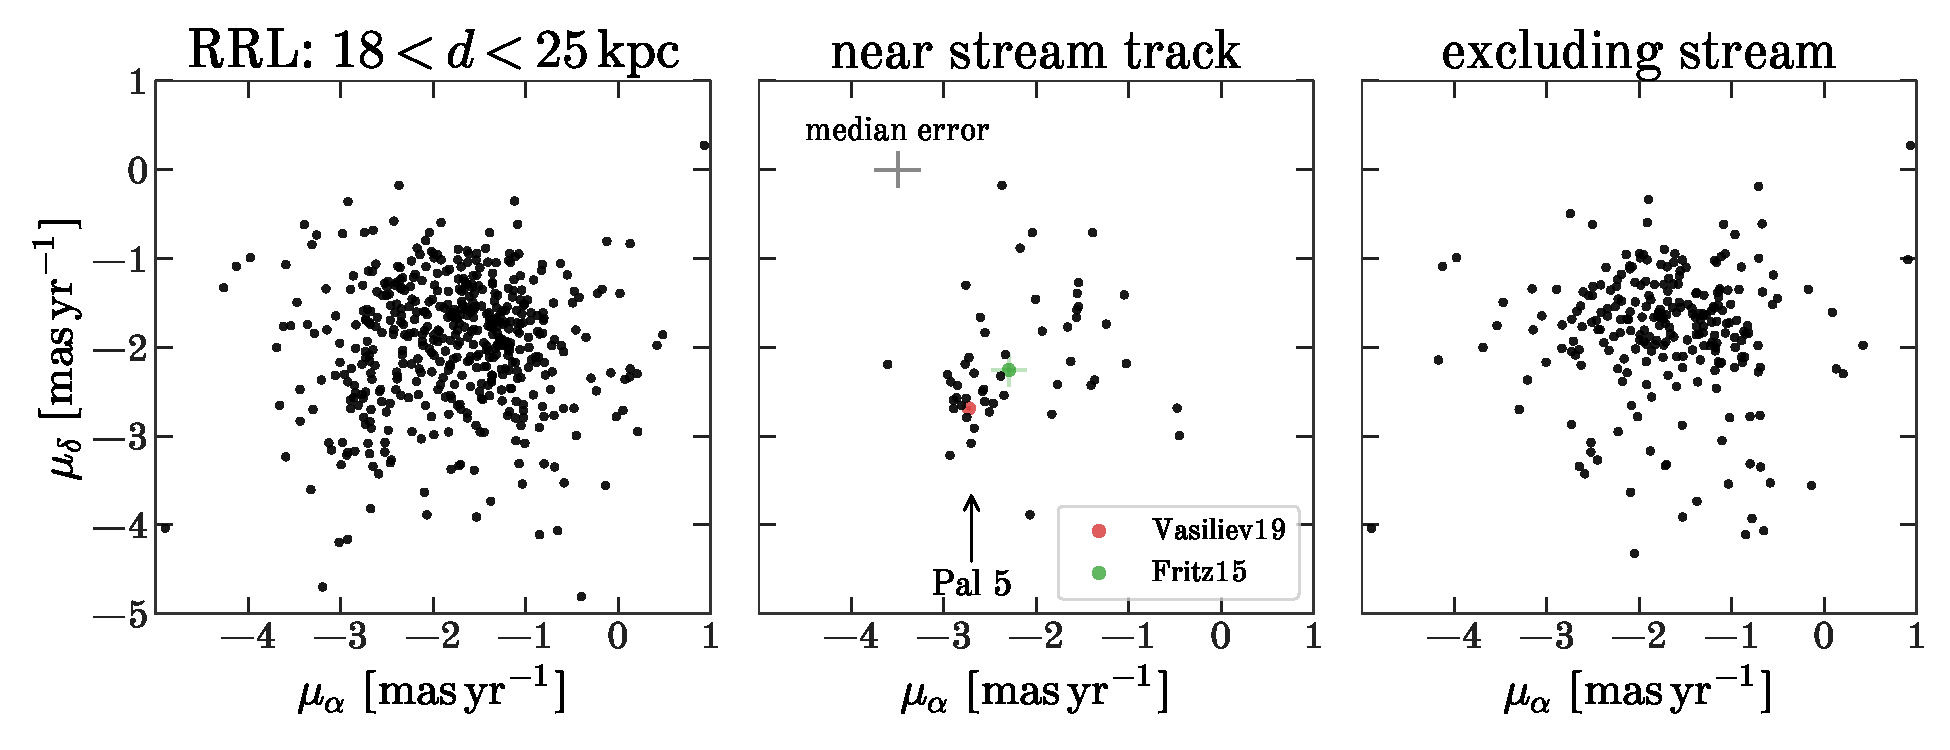
\includegraphics[width=\textwidth]{paper/proper-motion.pdf}
\caption{\textbf{Left}: Proper motions of RRLs in the region $215^\circ < \alpha < 255^\circ$, $-15^\circ < \delta < 10^\circ$ with distances in the range $18 < d < 25~\kpc$.
\textbf{Middle}: The same, but for RRLs within $1~\degr$ of the mean sky track of Pal 5 \citep{Bonaca:2019}.
The over-density of stars near $(-2.7, -2.7)$ is the stream, and the two colored points show the Pal 5 cluster proper motions from \citet{Vasiliev:2019} and \citet{Fritz:2015}, respectively.
\textbf{Right}: The same, but for RRLs excluding $2~\degr$ around the Pal 5 sky track.}
\label{fig:pm}
\end{center}
\end{figure*}

\section{Determining stream membership} \label{sec:membership}

In order to search for new RRL stars in the Pal 5 stellar stream, we construct a probabilistic model of the stream and background stellar distribution (simultaneously) using proper motion $(\mu_\alpha, \mu_\delta)$ and distance $d$ data for all RRL in the sky window $215^\circ < \alpha < 255^\circ$, $-15^\circ < \delta < 10^\circ$, where $(\alpha, \delta)$ are right ascension and declination.
We \emph{do not} include the known spatial extent or morphology of the Pal 5 stream in our membership model for the stream: We instead later use the sky positions to validate the modeling procedure and selection criteria we then use to define a sample of probable Pal 5 stream RRLs.
This model ultimately enables us to compute stream membership probabilities for RRL stars in a way that fully incorporates \Gaia\ error properties, while simultaneously modeling and marginalizing over uncertainties in the background RRL distribution.

To start, we use the sky track and width of Pal 5 from \citet{Bonaca:2019} to mask out a $\sim4^\circ$-wide region around the stream---and an extrapolation of the known extent of the stream---in order to define a ``background'' region that should be devoid of Pal 5 member stars.
\figurename~\ref{fig:pm} demonstrates that Pal 5 stream members appear in the RRL catalog: This figure shows the \Gaia\ \DR{2} proper motions for all RRLs in the sky window defined above within the distance range $18 < d < 25~\kpc$, then the same for RRLs in a tight selection around the observed stream track, and then finally the same for RRLs \emph{excluding} the stream region.
We use RRL stars in the background region to construct an error-deconvolved density model in the 3D space of proper motion components and distance.
We use proper motions and uncertainties from \Gaia---using the provided covariance matrix between proper motion components---and distances and uncertainties as derived above (\sectionname~\ref{sec:data}). 
We use \project{extreme deconvolution} \citep[\acronym{XD};][]{Bovy:XD} to optimize the parameters of a Gaussian Mixture Model (GMM) representation of the (deconvolved) background RRL density.
We first fit the background model (with \acronym{XD}) using between $3$--$12$ mixture components and evaluate the Bayesian Information Criterion (BIC) for the optimal parameters in each case.
From this, we find that the BIC is minimized for 6 mixture components: We therefore use 6 mixture components and fix the GMM model parameters to the \acronym{XD}-optimized values and use this as our background model.
We evaluate the background likelihood of all stars in the full sky region (defined above) and refer to this as $p_{{\rm bg}, n}$ (for the $n$th star) below.

To represent the Pal 5 stream, we use a single Gaussian component with a fixed dispersion of $0.05~\masyr$ for the proper motion components ($\approx 5~\kms$ at the distance of Pal 5) and $0.2~\kpc$ in distance.
However, we allow the mean to vary independently in each component as a function of $\phi_1$, a longitude coordinate (along the stream) as defined in \citet{Bonaca:2019}.
Based on the Pal 5 stream models from \citet{Bonaca:2019}, over the range of $\phi_1 \in (-20^\circ, 15^\circ$, the mean stream trends in $\mu_\alpha$, $\mu_\delta$, and distance can be well-approximated (within our observational uncertainties) by a quadratic function in $\phi_1$.
The mean of our stream component, $\bs{x}$, is therefore given by
\begin{equation}
    \bs{x} = \begin{pmatrix}
        \mu_\alpha^* + b_\alpha \, \phi_1 + c_\alpha \, \phi_1^2\\
        \mu_\delta^* + b_\delta \, \phi_1 + c_\delta \, \phi_1^2\\
        d^* + b_d \, \phi_1 + c_d \, \phi_1 \label{eq:meanpoly}
    \end{pmatrix}
\end{equation}
where $\bs{\theta} = (\mu_\alpha^*, \mu_\delta^*, d^*, b_\alpha, b_\delta, b_d, c_\alpha, c_\delta, c_d)$ are free parameters.

Given the above background model, and this model for the stream track, the full likelihood for an RRL star, $n$, with data $D_n = (\mu_\alpha, \mu_\delta, d)_n$ is represented as a mixture of the two components with mixture weight $f$,
\begin{equation}
    p(D_n \given \bs{\theta}, f) = f \, \mathcal{N}(D_n \given \bs{x}, \mat{C}) + (1-f)\,p_{{\rm bg}, n}
\end{equation}
where $\mathcal{N}(\cdot \given \bs{x}, \mat{C})$ is the multivariate normal distribution with mean $\bs{x}$ and covariance matrix $\mat{C}$.

We use Markov Chain Monte Carlo (MCMC) to generate samples over the parameters $(\bs{\theta}, f)$ using the posterior probability
\begin{equation}
    p(\bs{\theta}, f \given \{D_n\}) \propto p(\bs{\theta}, f) \, \prod_n^N p(D_n \given \bs{\theta}, f)
\end{equation}
where $p(\bs{\theta}, f)$ is the prior probability distribution over the parameters.
We assume that our prior is separable in all of our parameters: We use a uniform prior for the mixture weight, $f$, such that $p(f) = \mathcal{U}(0, 1)$, Gaussian priors on the mean proper motion and distance using the Pal 5 cluster proper motion measurements from \citet{Vasiliev:2019} and the Pal 5 distance from \citet{Kuepper:2015}.
We use broad uniform priors on the linear and quadratic polynomial coefficients defined in \equationname~\ref{eq:meanpoly}.
We use the affine-invariant ensemble MCMC sampler \texttt{emcee} \citep{emcee} to sample from the posterior probability distribution given above.
We run \texttt{emcee} with 80 walkers for an initial 1024 steps to ``burn-in'' the sampler, then reset and restart the sampler for another 2048 steps.
We compute the Gelman-Rubin convergence statistic $\mathcal{R}$ \citep{Gelman:1992} to verify that $\mathcal{R} < 1.1$ for all walkers and assume that the chains have converged.
We then thin the chains by saving only every 128th step, leaving us with 1,280 posterior samples in our membership model parameters, $\bs{\theta}$.
For each star, we also compute posterior membership probabilities using the samples following \citet{DFM:blog}.

\figurename~\ref{fig:trackmembers} shows a summary of the inferred membership model properties in sky position (shown in Pal 5 coordinates $\phi_1, \phi_2$), distance, and proper motion components.


\begin{figure*}[t]
\begin{center}
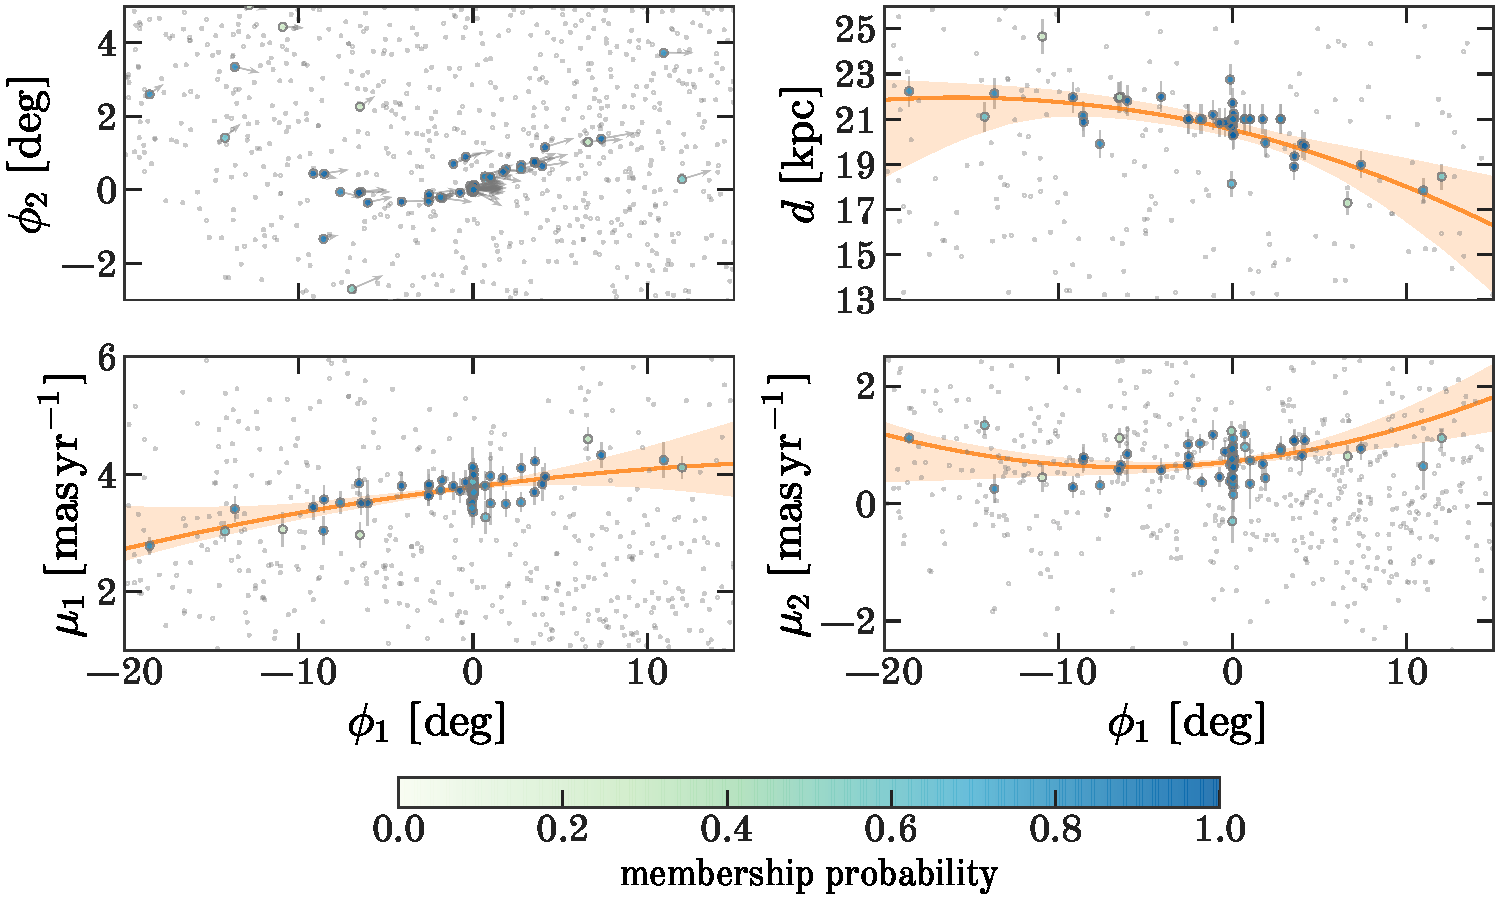
\includegraphics[width=\textwidth]{paper/tracks.pdf}
\caption{RRL stars in the vicinity of the Pal 5 stream (with $\textrm{prob.} > 0.01$), colored by membership probability, and under-plotted with the inferred stream trends used in the membership model.
\textbf{Upper left}: Sky positions (in the Pal 5 stream coordinate frame) of RRLs, with arrows showing the \Gaia\ \DR{2} proper motion vector direction.
\textbf{Upper right}: Distance as a function of Pal 5 longitude, $\phi_1$, for the RRLs. The shaded (orange) band shows the 16--84th percentile confidence region for the inferred distance trend of the stream, and the solid line shows the median posterior sample, all assuming a quadratic function of $\phi_1$.
\textbf{Lower panels}: Same as upper right, but for the proper motion in right ascension, $\mu_\alpha$, and declination, $\mu_\delta$.
}
\label{fig:trackmembers}
\end{center}
\end{figure*}


\section{Results} \label{sec:results}

\begin{figure*}[t]
\begin{center}
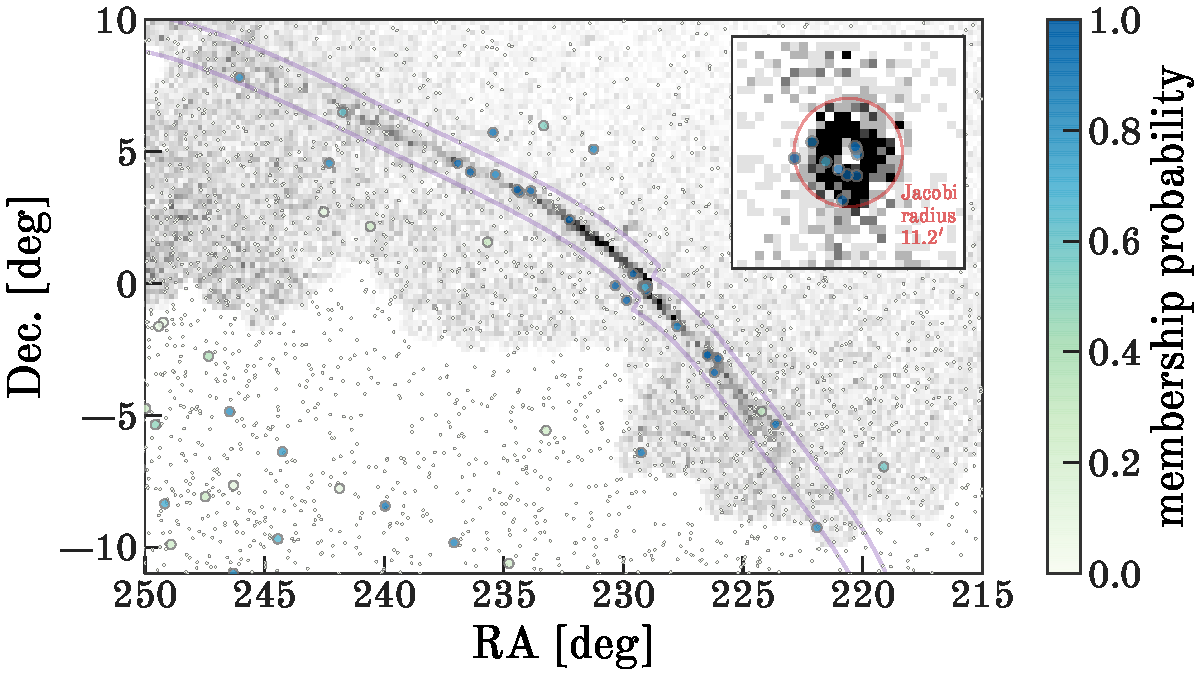
\includegraphics[width=\textwidth]{paper/members.pdf}
\caption{Sky positions of RRL...todo}
\label{fig:members}
\end{center}
\end{figure*}

\subsection{RR Lyrae stars associated with Pal 5 and its tails}

\todo{How many we find, what their types are}


\subsection{Kinematics of the stream and cluster}

\todo{Summarize mean dist and pm from RRLs, and trend parameters}

\todo{Make a table with summary information}



\subsection{RR Lyrae stars known to be associated with Pal 5 or it's tails}

\todo{move some of this to discussion?}

Pal~5 has 5 known RRL stars (V1-V5), all of type \typec, as reported in the \citet{Clement2001} compilation of variable stars in Galactic globular clusters and dating back to \citet{SawyerHogg1973}. Star V2 has a  systemic radial velocity of  $-65\pm16$~\kms~measured by \citet{Vivas2005}. 

In their analysis of the halo density profile \citet{Vivas2006} report an overdensity, dubbed Group~6, containing 6 previously unidentified RRLs. Based on the distance to the RRLs they claim many of these could be associated to Pal~5's tidal tails. The QUEST IDs of the stars in their Group~6 are: 403, 405, 407, 411, 416 and 422. The first two stars --403 and 405-- are located at distances of  $9\farcm8$ and $11'$ from the cluster's center, which \citet{Vivas2004} notes places them within the cluster's tidal radius, assuming the value of $r_t\sim16'$ reported by \citet{Odenkirchen:2002}.  \todo{Update this value}. \citet{Vivas2006} also note that star 393, not in Group~6, could also be associated to the cluster's tails, given it's distance and location along the known extent of the tails.

In summary,  previous studies report 7 known RRLs associated to the cluster itself (1 \typeab~and 6 \typec) plus 5 more reported as possibly associated to the tails (4 \typeab~and 2 \typec). 

% 
\begin{table*}[t]
\caption{RRL members of the Pal 5 stream.}\label{t:rrl_members}
\begin{footnotesize}
\begin{tabular}{llllllll}
\toprule
\Gaia~DR2               & Other & Period & Amp-$g$ & Type & D & member & sep  \\
\verb+source_id+        & ID   & (d)    & (mag)   &     &(kpc)& prob & (") \\
\midrule
4418920808077110784 &  V5 & 0.337934& 0.46 & RRc  & 20.73 & 0.9982 &   1.9 \\
4418920846732620032 &     & 0.643239& 0.27 & RRab & 21.71 & 0.9963 &   2.0 \\
4418914863842345856 &  V1 & 0.293229& 0.56 & RRc  & 20.36 & 0.9696 &   2.0 \\
4418726027016125056 &  V3 & 0.329948& 0.51 & RRc  & 20.65 & 0.9978 &   3.8 \\
4418725889577171328 &  V4 & 0.286366& 0.59 & RRc  & 20.28 & 0.9915 &   4.5 \\
4418731829516302848 &     & 0.28164 & 0.3  & RRc  & 18.14 & 0.9297 &   4.8 \\
4418913218870688768 &  V2 & 0.332473& 0.4  & RRc  & 20.33 & 0.9977 &   5.0 \\
4418734165978521728 &     & 0.380859& 0.52 & RRc  & 22.75 & 0.9850 &   7.6 \\
4418724034151291776 & 403 & 0.551705& 1.14 & RRab & 21.23 & 0.9987 &   9.7 \\
4418732791593809152 & 405 & 0.329670& 0.45 & RRc  & 20.74 & 0.9959 &  11.0 \\
4419052204012341760 &     & 0.530006& 1.01 & RRab & 20.84 & 0.9960 &  44.5 \\
4418142117622280192 & 393 & 0.462671& 1.36 & RRab & 19.95 & 0.9060 & 118.7 \\
6339498589346000768 &     & 0.320110& 0.46 & RRc  & 18.89 & 0.9934 & 217.7 \\
6339499379619987200 &     & 0.329577& 0.47 & RRc  & 19.35 & 0.9966 & 218.6 \\
6339478312804685824 &     & 0.465883& 1.12 & RRab & 19.91 & 0.9970 & 242.8 \\
4421078432143578496 &     & 0.520749& 1.11 & RRab & 21.98 & 0.9981 & 246.1 \\
6339398155830632448 &     & 0.688316& 0.75 & RRab & 19.82 & 0.9982 & 258.9 \\
4427253907921168000 &     & 0.496334& 1.35 & RRab & 21.81 & 0.9905 & 362.5 \\
4427220338456828416 &     & 0.600796& 0.81 & RRab & 21.98 & 0.9974 & 384.4 \\
4427234700827469952 &     & 0.517911& 1.24 & RRab & 21.94 & 0.9979 & 392.3 \\
6337302795905934336 &     & 0.519462& 1.02 & RRab & 17.29 & 0.9808 & 404.5 \\
6337233350579111680 &     & 0.542383& 0.96 & RRab & 18.98 & 0.9962 & 450.6 \\
4427646704153765632 &     & 0.385552& 0.37 & RRc  & 19.90 & 0.9429 & 456.5 \\
4424705647988505600 &     & 0.335502& 0.41 & RRc  & 20.87 & 0.9832 & 513.0 \\
4426221707021159424 &     & 0.533313& 1.14 & RRab & 21.97 & 0.9728 & 550.1 \\
\bottomrule
\end{tabular}
\end{footnotesize}
\end{table*}

\subsubsection{Notes on individual stars}

Star 422 is reported as an \rrc~in \citet{Vivas2004}, with a period of 0.61925~d and $V$ amplitude 0.51~mag. In PS1 it is classified as an \rrc~with a period of 0.3832276153~d. The period reported in \citet{Vivas2004} is an alias of this one, more likely to be the true period given the variability amplitude\footnote{\citet{Vivas2004} also cautions that derived periods for QUEST \rrc~stars are known to be prone to aliasing due to the observing cadence of $\sim1$~d.}. Therefore, we keep PS1's classification henceforth for RRL 422.  

Star \verb+source_id=6339498589346000768+ is reported both in PS1 and \Gaia~as an \rrc~, with a period 0.4714315854~d in PS1 and 0.320110123108~d in \Gaia~SOS, the two are a pair of 1~d aliases \citep[see e.g.]{Lafler1965}. In what follows we adopt the shorter period reported in \Gaia~as the correct one as it is the more probable one for an \rrc~star.

Star \verb+source_id=4418731829516302848+ is reported in PS1 and \Gaia~as an \rrab~with a period around 0.646 and a similarly low amplitude $A_G=0.2$ and $A_g=0.3$ in both surveys. This star is reported in CRTS \citep{Drake2014} (ID CSS\_J151623.2-000831) as an \rrc~with a period 0.28164~d. We adopt the CRTS period for this star in what follows, as it is based on many more observations ($\gtrsim200$) than \Gaia~and PS1's (about a dozen per filter in each case) and the \rrc~classification and short period are more likely for such a short amplitude star.  


\subsection{RR Lyrae population }

Based on the paucity of RRL stars of type~\typeab~in the cluster, Pal~5  would have been expected to be classified as an Oosterhoff type II cluster (ref-XX, no one really seems to say this explicitly), at odds with the cluster's known spectroscopic metallicity of $\FeH=-1.32$ \citep{Kuijsen2018}, as OoII clusters are on average more metal-poor than OoI clusters.

We find 15 RRLs in the cluster tails, $\sim11$ of \type~ab and $\sim4$ of \type~c. Combined with the 10~\rrc~in the cluster itself, there are 25 RRLs in total associated to Pal~5 and its tails with membership probabilities larger than 0.5. Figure~\ref{fig:PA_diagram} shows the period-amplitude diagram for the RRL stars in Pal~5. The full sample of PS1 RRLs is shown in the background for comparison, as a grayscale density histogram. The distribution of the \typeab~RRL clearly indicate Pal~5 to be an Oosterhoff I cluster, consistently with their mean period of 0.565~d(XX).  Our findings of the updated ratio of \rrab~to~\rrc, mean period and Period-Amplitude distribution of the \rrab, all support an OoI classification for Pal~5, consistent with the cluster's metallicity.

Out of our newly found \rrab's three are High Amplitude Short Period (HASP, $P <0.48$~d, $A_V>0.75$~mag $=A_g>$) stars. This type of RRL is only found in relatively metal-rich globular clusters  \citep[$\Feh>-1.5$][]{Monelli2017} and the Sagittarius dwarf galaxy, but not in any other dwarf spheroidal galaxy. \todo{CM:( any other point to be made about this?)}.


\begin{figure}
\begin{center}
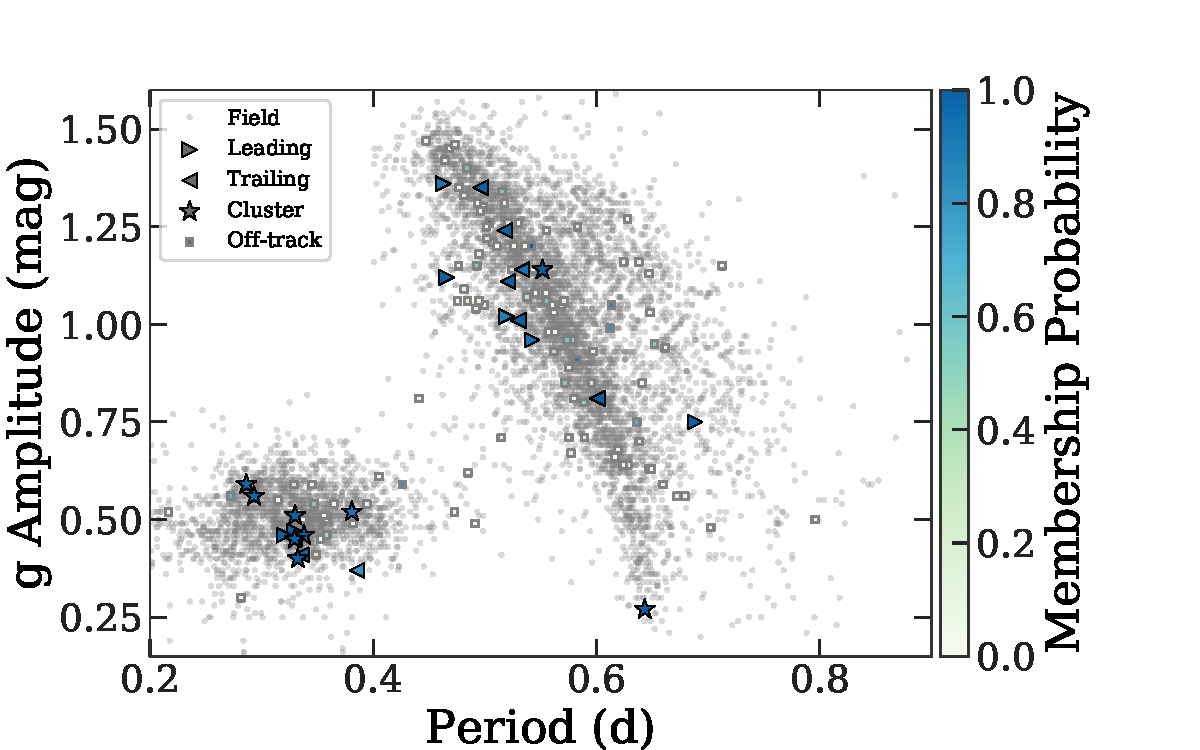
\includegraphics[width=\columnwidth]{paper/rrls_PA.pdf}
\caption{Amplitude ($g$-band) versus Period for RRLs in the Pal~5 field.}\label{fig:PA_diagram}
\end{center}
\end{figure}

\subsection{Stellar Mass and Luminosity}

%We can provide an estimate on the cluster's luminosity based on the observed number of RRLs. For that, the first step is to assess how complete our observed sample is. 

\citet{Sesar2017b} provide an estimate of their catalogue's completeness as a function of distance, at high galactic latitude, based on simulations. They estimate the mean completeness to be 92\% for \rrab~and 79\% for \rrc, up to a distance of 40~kpc, well beyond the distance of Pal~5 and its tails. At the average ratio of 3 \rrc~stars per every 10 \rrab~\citep{Layden1995}, this represents a mean completeness of 89\%. We can also produce an estimate per line of sight using the methodology described in \citet{Rybizki2018}, which requires two independent catalogues to assess the completeness of both in a probabilistic manner. Using the \Gaia~DR2 VariClassifier \citet{Holl2018,Rimoldini2018} and Specific Objects Study \citep{Clementini2018} catalogues, we find a median completeness of 92\% with a standard deviation of 16\%  with no evident spatial trend across the field of Figure~\ref{fig:members}.

%we obtain the completeness map shown in Figure~\ref{fig:completeness_map}, for RRLs of type \typeab~and \typec. The mean completeness estimated this way is 92\% with a standard deviation of 16\% and, as the figure shows, there is no evident spatial trend. The two estimates are remarkably consistent and, in what follows, we will adopt a completeness of 90\%-XX.

To estimate the expected absolute magnitude of Pal 5 we follow the same procedure as in \citet{Mateu2018}, who use a linear fit of the relation between the absolute magnitude $M_V$ and the number of \typeab RRL, based on data from Galactic dwarf galaxies and globular clusters. Here we use it including the data for the \typec~stars.
Correcting the observed number of 25~RRLs by the median completeness of 92\%, we get a total expected number of 28~RRLs, for which find an absolute magnitude $M_V=-8.1\pm 1.1$.

% \begin{figure}
% \begin{center}
% 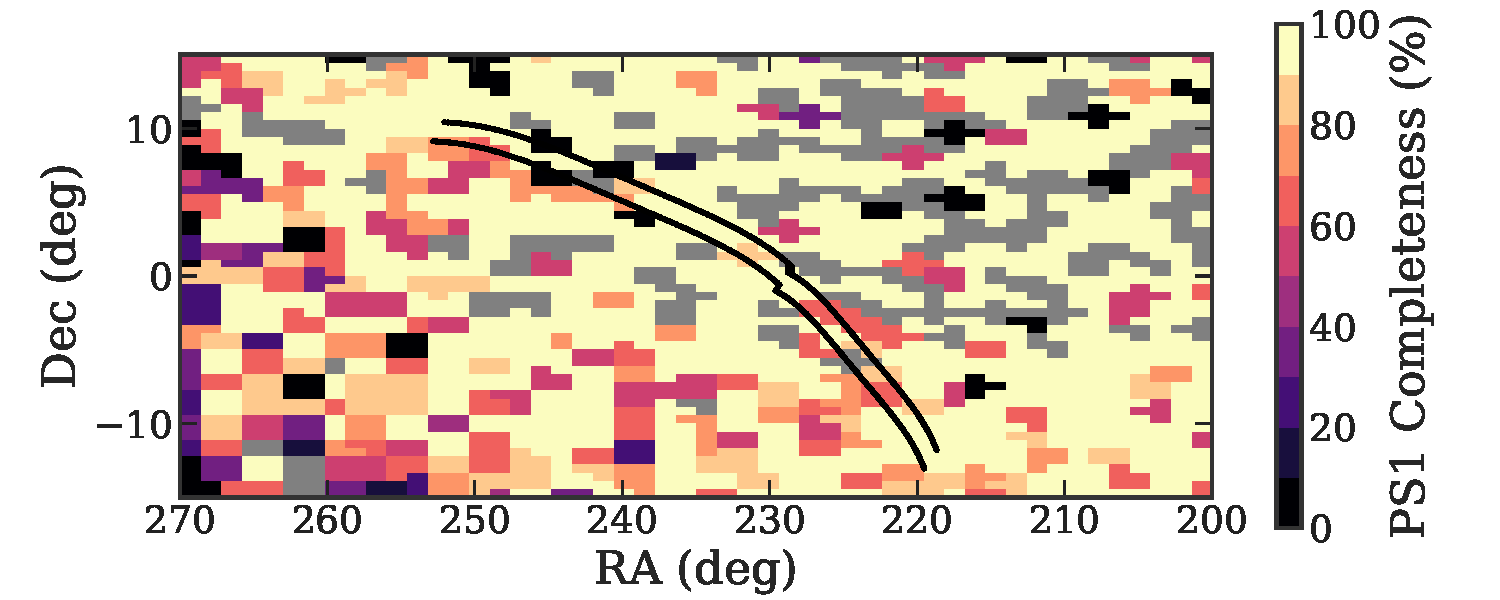
\includegraphics[width=\columnwidth]{paper/ps1_completeness.pdf}
% \caption{PS1 RRL estimated completeness. The Pal 5 stream's track is shown with the solid line.}\label{fig:completeness_map}
% \end{center}
% \end{figure}

\todo{CM: estimate luminosity based on number of RRLs. Compare to estimate from $M_V-\Feh$ relation. Derive stellar mass from stellar luminosity. Compare to dynamical mass estimates.}


- there are $\sim4$-XX times as many RRLs in the tails as there are in the cluster.  
- how much mass did we already know to be in the tails compared to the cluster? (\sa{according to Ibata 2016 the mass in the present day cluster is 4297 $\pm~ 98$ M$_{\odot}$, and the streams excluding the cluster have $\sim$7903 M$_{\odot}$. So under a factor of 2 more stars in the tails than in the remnant cluster}. The cluter is thought to have had an initial mass of $\sim47000$ M$_{\odot}$). Probably not as much as a factor of 4. This makes it unexpected to have found this many RRLs in the tails. Based on prior knowledge of the mass loss undergone by the cluster we would have expected this to be XX (Sarah?/Adrian?) \sa{Not sure, the lowest mass stars should have been lost first...}. Similarly, 




\subsection{Implications for stellar population}

\todo{Constraints on initial mass of Pal 5}

\todo{CM:} Inferred luminosity based on the number of RRLs is XX. Compare to inferred luminosity based on the $M_V-\FeH$ relation. 

\subsection{Cluster distance and stream track}


\software{
    Astropy \citep{astropy, astropy:2018},
    emcee \citep{emcee},
    gala \citep{gala},
    IPython \citep{ipython}
}

\bibliographystyle{aasjournal}
\bibliography{refs,cm1,cm2}

\end{document}
